\documentclass{article}
\usepackage{amsmath, amssymb, cancel, mathtools, bm}
\usepackage[left=.5in, right=.5in, top=1in, bottom=1in]{geometry}
\usepackage[most]{tcolorbox}
\usepackage[skip=1em,indent=0pt]{parskip}
\setlength{\parindent}{0pt}
\newcommand{\statvec}[1]{\underset{\sim}{\bm{#1}}} % Vector symbol (tilde under vector)
\DeclareMathOperator{\EX}{\mathbb{E}} % Expected Value symbol
\newcommand{\indep}{\perp\!\!\!\!\perp} % Independence symbol
\newcommand{\real}{\mathbb{R}} % Simplified 'Reals' indicator
\newcommand{\pto}{\overset{P}{\to}}
\newcommand{\asto}{\overset{a.s.}{\to}}
\newcommand{\rthto}{\overset{L^r}{\to}}
\newcommand{\dto}{\overset{D}{\to}}
\newcommand{\ext}{\EX_{\theta}}
% Force all aggregate symbols to always put values above/below
\let\Oldint=\int
\let\Oldsum=\sum
\let\Oldprod=\prod
\let\Oldbigcup=\bigcup
\let\Oldbigcap=\bigcap
\let\Oldlim=\lim
\renewcommand{\int}{\Oldint\limits} 
\renewcommand{\sum}{\Oldsum\limits} 
\renewcommand{\prod}{\Oldprod\limits} 
\renewcommand{\bigcup}{\Oldbigcup\limits} 
\renewcommand{\bigcap}{\Oldbigcap\limits} 
\renewcommand{\lim}{\Oldlim\limits} 
\newcommand{\infint}{\int_{-\infty}^{\infty}}
\newcommand{\iiddist}{\overset{\mathrm{iid}}{\sim}}
\newcommand{\norm}[1]{\left\lVert#1\right\rVert}
\newcommand{\boldred}[1]{\textbf{\textcolor{red}{#1}}}


\begin{document}

\section{CB2 10.34}

Testing $X_i \iiddist Bern(p); H_0: p = p_0, H_1: p \neq p_0$

(a) Derive expression for $-2ln(\lambda(x))$

$L(p|X) = \prod p^x(1-p)^{1-x} = p^{\sum x}(1-p)^{n-\sum x}$

Under the null, $\hat{p}_R = p_0$. Unrestricted, $\hat{p} = \bar{x}$

LRT: $\lambda(x) = \frac{L(\hat{p}_R|x)}{L(\hat{p}|x)} = \frac{p_0^{\sum x}(1-p_0)^{n-\sum x}}{\bar{x}^{\sum x}(1-\bar{x})^{n-\sum x}} = \left(\frac{p_0}{\bar{x}}\right)^{\sum x}\left(\frac{1-p_0}{1-\bar{x}}\right)^{n-\sum x} = \left(\frac{p_0(1-\bar{x})}{\bar{x}(1-p_0)}\right)^{\sum x}\left(\frac{1-p_0}{1-\bar{x}}\right)^n$

$$
\begin{aligned}
-2ln(\lambda(x)) 
& = -2 ln(\left(\frac{p_0(1-\bar{x})}{\bar{x}(1-p_0)}\right)^{\sum x}\left(\frac{1-p_0}{1-\bar{x}}\right)^n) \\
& = -2 [\sum(x) ln\left(\frac{p_0(1-\bar{x})}{\bar{x}(1-p_0)}\right) + n ln\left(\frac{1-p_0}{1-\bar{x}}\right)] \\
& = -2\left[\sum x \left(ln(p_0) + ln(1-\bar{x}) - ln(\bar{x}) - ln(1-p_0)\right) + n\left(ln(1-p_0) - ln(1-\bar{x})\right)\right]
\end{aligned}
$$

(b) Simulate distribution of $-2ln(\lambda(x))$ and compare to the $\chi^2$ approximation. 

Using the following code: 

\begin{verbatim}
two_log <- function(x, p0) {
  n <- length(x)
  x_bar <- mean(x)
  sum_x <- sum(x)
  -2 * (sum_x*(log(p0) + log(1-x_bar) - log(x_bar) - log(1-p0)) + n*(log(1-p0) - log(1-x_bar)))
}

p0 <- .25

n_sim <- 10000
n <- 10
res <- numeric(n_sim)
for (i in 1:n_sim) {
  x <- rbinom(n = n, size = 1, prob = p0)
  res[i] <- two_log(x, p0)
}

hist(res, freq = FALSE)
curve(dchisq(x, df = 1), add = TRUE, col = 'red')
\end{verbatim}

I got: 

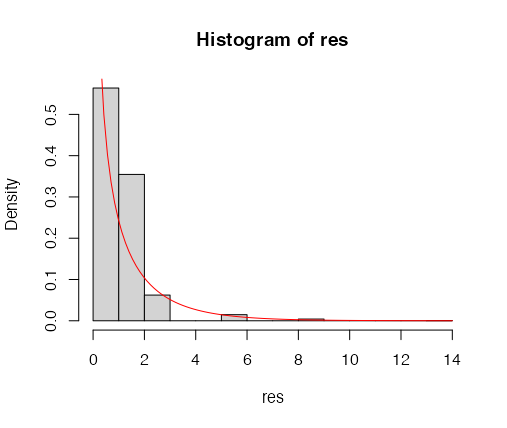
\includegraphics{hw9_1_b.png}

\section{CB2 10.36, 10.38} (omit part(c))

$X_i \iiddist Gamma(\alpha, \beta), \alpha$ known, $\beta$ unknown. $H_0: \beta = \beta_0, H_1: \beta \neq \beta_0$

10.36 (a) What is the MLE of $\beta$?

$L(\beta|\alpha, x) = \prod \frac{\beta^{\alpha}}{\Gamma(\alpha)} x^{\alpha-1} e^{-\beta x} = \frac{\beta^{n \alpha}}{\Gamma(\alpha)^n}\prod(x^{\alpha-a})e^{-\beta \sum x}$

$l(\beta|\alpha, x) = \sum ln(\frac{\beta^{\alpha}}{\Gamma(\alpha)} x^{\alpha-1} e^{-\beta x}) = \sum [\alpha ln(\beta) - ln(\Gamma(\alpha)) + (\alpha-1)ln(x) - \beta x] = n \alpha ln(\beta) - n ln(\Gamma(\alpha)) - \beta \sum x + (\alpha - 1)\sum ln(x)$

$\frac{\partial l}{\partial \beta} = \frac{n\alpha}{\beta} - \sum x = 0 \implies \beta = \frac{n \alpha}{\sum x} = \frac{\alpha}{\bar{x}}$

10.36 (b) Derive Wald statistic for testing $H_0$ using the MLE in both the numerator and denominator of the statistic.

$Z_w = \frac{\sqrt{n}(\hat{\beta} - \beta)}{\sqrt{1/I_1(\hat{\beta})}}$

$I_1(\hat{\beta}) = \frac{\partial l^2}{\partial \beta^2} = \frac{\partial}{\partial \beta} \frac{\alpha}{\beta} - \sum x = -\frac{\alpha}{\beta^2}$

$Z_w = \frac{\sqrt{n}(\hat{\beta} - \beta)}{\sqrt{\hat{\beta}^2/\alpha}} = \frac{\sqrt{n}(\frac{\alpha}{\bar{x}} - \beta)}{\sqrt{\frac{\alpha^2}{\bar{x}^2\alpha}}} = \frac{\sqrt{n}(\frac{\alpha}{\bar{x}} - \beta)}{\frac{\sqrt{\alpha}}{\bar{x}}}$

10.38: Derive a score statistic for testing $H_0$.

$Z_s = \frac{\psi(x;\hat{\beta})}{\sqrt{n I_1(\hat{\beta})}}$

$\psi(\hat{\beta}) = \frac{n\alpha}{\hat{\beta}} - \sum x$

$Z_s = \frac{\frac{n\alpha}{\hat{\beta}} - \sum x}{\sqrt{n}\sqrt{\hat{\beta}^2/\alpha}} = \frac{\frac{n\alpha}{\frac{\alpha}{\bar{x}}} - \sum x}{\sqrt{n}{\sqrt{\frac{\alpha^2}{\alpha \bar{x}}}}} = \frac{n\bar{x} - \sum x}{STUFF} = \frac{\sum x - \sum x}{STUFF } = 0$

\section{CB2 9.13}

$X_1 \sim Beta(\theta,1)$

(a)

$Y = -(ln(X))^{-1}$. Evaluate confidence coefficient of the set $[y/2, y]$.

$\implies -\frac{1}{Y} = ln(X) \implies X = e^{-1/Y} \implies \frac{dx}{dy} = \frac{1}{y^2}e^{-1/y}$

$f(X) = \frac{\Gamma(\theta)}{\Gamma(\theta + 1)}x^{\theta-1} = \theta x^{\theta-1}$

$f(Y) = \theta (e^{-1/y})^{\theta-1}\frac{1}{y^2}e^{-1/y} = e^{1/y - \theta/y - 1/y}\frac{\theta}{y^2} = \frac{\theta}{y^2}e^{-\theta/y}$

We want to find: $P(y/2 \le \theta \le y) = P(\theta \le Y \le 2\theta) = \int_{\theta}^{2 \theta} \frac{\theta}{y^2}e^{-\theta/y} dy = e^{-\theta/y}|_{\theta}^{2\theta} = e^{-1/2}- e^{-1} \approx .239$

(b) 

Find a pivotal quantity and use it to set up a confidence interval have the same conidence coefficient as the interval in part (a)

$f(x) = \theta x^{\theta-1}$. This has the parameter in the exponent, so we'll start with $X^\theta$ as our pivot. 

I got help on this part: apparently $X^{\theta} \sim U(0,1)$ (not sure how we derive that). However, that means that $P(a \le X^\theta \le b) = b-a$, which will give a confidence coefficient of $b-a$. So, as long as we set $b-a = .239$ it has the same confidence coefficient as part (a). 

(c)

Compare the expected value of the length of each interval

If we minimize the length of the pivotal interval in (b), we want to minimize $ln(b)-ln(a)$ conditioned on $b - a = 1-\alpha \implies b = 1-\alpha + a \implies$ we want to minimize $ln(1-\alpha+a) - ln(a) = ln(\frac{1-\alpha + a}{a}) = ln(1 + \frac{1-\alpha}{a})$. We minimize this by making a big. To make a as big as possible (bounded by $b-a=1-\alpha$, and $b, a, <1$) we have to set $b = 1, a = \alpha$. Thus our minimum interval becomes: 

$\{\theta: 0 \le \theta \le \frac{ln(\alpha)}{ln(x)}\}$

For part (a): This is a special case of the above interval, but with the restriction that $b = 2a$. Unless $\alpha = .5$, this interval will end up being wider than the minimum interval described above. 

Thus, except in one specific scenario, part (a) will have a wider interval than part (b.)

\section{CB2 9.17}

Use a pivot method to find these intervals, not inverting tests

Find a $1-\alpha$ confidence interval for $\theta$ given $X_i \iiddist$...

(a) $f(x|\theta) = 1, \theta - \frac{1}{2} < x < \theta + \frac{1}{2}$

This is just a uniform over $x$ centered on $\theta$. So, if we take out pivot to be $X-\theta$, that gives us a $U(-\frac{1}{2}, \frac{1}{2})$ distribution. 

That gives us $P(a \le X-\theta \le b) = b-a$, and we have the constrant $b-a = 1-\alpha \implies b = 1-\alpha + a$. 

We can then just pick any $a, b$ which satisfy $b = 1-\alpha + a$ (bounded by $-1/2, 1/2$).

(b) $f(x|\theta) = \frac{2x}{\theta^2}, 0 < x < \theta, \theta > 0$

This is a scale parameter, so we'll go with $T = \frac{X}{\theta}$, which has PDF of $f(t) = 2t, 0 \le t \le 1$. 

Thus, $P(a \le \frac{X}{\theta} \le b) = \int_a^b 2tdt = t^2|_a^b = b^2 - a^2$

Thus, we cna pick any values for $a,b$ which satisfy $b^2 - a^2 = 1-\alpha$

\section{CB2 9.4}

$X_i \iiddist N(0, \sigma_x^2), Y_i \iiddist N(0, \sigma_y^2), \lambda = \frac{\sigma_y^2}{\sigma_x^2}$

(a) Find the level $\alpha$ of $H_0: \lambda = \lambda_0, H_1: \lambda \neq \lambda_0$

I'm not gonna lie: I looked at the solution for this problem and this looks aboslutely wild. 

The very basics follow the same process as in other problems: Use the unrestricted MLEs ($frac{\sum x_i^2}{n}, \frac{\sum y_i^2}{m}$), with the restricted being $\hat{\lambda} = \lambda_0 \implies \sigma^2_Y = \lambda_0 \sigma^2_X$

Which you can then plug into the likelihood to get $\hat{\sigma}^2_0 = \frac{\lambda_0 \sum x_i^2 + \sum y_i^2}{\lambda_0 (m+n)}$

Which you can then plug into the LRT: $\frac{L(\lambda_0, \hat{\sigma}^2_0|X,Y)}{L(\hat{\sigma}^2_X, \hat{\sigma}^2_Y|X,Y)} = \frac{\hat{\sigma}_X^n \hat{\sigma}_Y^m}{\lambda_0^{m/2} \hat{\sigma}_0^{(m+n)}}$

This then gives the rejection test to reject when $\lambda < k$ where k is picked to give size $\alpha$.

(b) Express rejection region of the LRT from (a) in terms of an F random variable

This is the part that looked particularly crazy when viewing the solution. Honestly, wild. 

Somehow we're supposed to recognize that $F = \frac{\frac{\sum y_i^2}{\lambda_0 m}}{\frac{\sum x_i^2}{n}} \sim F_{m,n}$ which we could then use to form a rejection region. 

(c) Find a $1-\alpha$ confidence interval for $\lambda$

Even looking at the solution, I can't really tell what the solution is doing haha. This question just kind of all went over my head. 

\section{CB2 9.36}

$X_i \iiddist f_{X_i}(x|\theta) = e^{i\theta - x}I_{[i\theta, \infty)}(x)$. Prove that $T = min_i(X_i / i)$ is a sufficient statistic for $\theta$. Based on T, find the $1-\alpha$ confidence interval for $\theta$ interms of $[T+a, T+b]$ which is of minimum length. 

The indicator portion $I_{[i\theta, \infty)}(x)$ can be rewritten as $I_{[\theta, \infty)}(x/i)$. In order for this indicator to be active for all X's (for the likelihood), we just need to know that the smallest x value is within that range, meaning that indicator is a function of $min_i(X_i/i)$. Thus, we can write the original PDF as $e^{-x}e^{i\theta}I_{[\theta, \infty)}(min_i(X_i/i)) = h(x)g(T, \theta)$ thus $T$ is a sufficient statistic. 

$L(\theta|x) = e^{\sum(-\theta - x)}I_{[\theta, \infty)}(min_i(X_i/i))$

$P(T > t) = \prod P(X_i > it) = \prod \int_{it}^{\infty}e^{i\theta - x}dx = \prod [-e^{i\theta-x}]|_{it}^{\infty} = \prod [0 - (-e^{i\theta - it})] = \prod e^{i(\theta-t)} = \text( had to get some help here ) = e^{-\frac{n(n+1)}{2}(t-\theta)}$

Thus, $f_T(t) = \frac{n(n+1)}{2}e^{-\frac{n(n+1)}{2}(t-\theta)}$

This is a location family, so the pivot would be $T_\theta$. We need to minimize $[T+a, T+b]$, so we need to minimize $b-a$ subject to $P(-b \le T-\theta \le -a) = 1-\alpha$. $T-\theta$ is monotonically decreasing, so the shortest length when $b=0$ is $P(0 \le T-\theta \le -a) = e^{-\frac{n(n+1)}{2}a} = 1-\alpha \implies -\frac{n(n+1)}{2}a = ln(1-\alpha) \implies a = -\frac{2ln(1-\alpha)}{n(n+1)}$

Smallest interval is $[T+(-\frac{2ln(1-\alpha)}{n(n+1)}), T]$

\section{}

$Y_i \iiddist U(0, \theta)$. Find the $1-\alpha$ pivotal interval based on $Y_{(n)}$ that is of the shortest length.

This is actually a scale parameter, so $\frac{T}{\theta}$ is our pivot. CDF of pivot is $F(t) = (\frac{t\theta}{\theta})^n = t^n, f(t) = n t^{n-1}$

We will have an interval of $[aT, bT]$, and want to minimize $b-a$ such $P(a \le \frac{T}{\theta} \le b) = 1-\alpha$

$\frac{T}{\theta}$ is monotonically decreasing, so letting $a = 1$ $P( a \le \frac{T}{\theta} \le b) = P(\frac{T}{b} \le \theta \le \frac{T}{a}) = 1-\alpha$

Length: $L = T(\frac{1}{a} - \frac{1}{b})$. Need to minimize width under $P(a \le \frac{T}{\theta} \le b) = 1-\alpha$.

$f(t)$ is an increasing function, so we'll set $b=1$: $P(\frac{T}{\theta} < a) = a^n = \alpha \implies a = \alpha^{1/n}$

Thus our interval is: $[T, \frac{T}{a^{1/n}}]$

\section{CB2 9.6}

Part (a) only

(a) Find the $1-\alpha$ confidence set for a binomial $p$ by inverting the LRT of $H_0: p = p_0, H_1: p \neq p_0$

$L(p|x) = \prod \binom{n}{x} p^x (1-p)^{n-x} = \prod [\binom{n}{x}] p^{\sum x} (1-p)^{n - \sum x}$

For a binomial, $\hat{p} = \bar{x} = \frac{\sum x}{n}$

$\lambda(x) = \frac{L(p_0|x)}{L(\hat{p}|x)} = \frac{\prod [\binom{n}{x}] p_0^{\sum x} (1-p_0)^{n - \sum x}}{\prod [\binom{n}{x}] \hat{p}^{\sum x} (1-\hat{p})^{n - \sum x}} = (\frac{p_0}{\hat{p}})^{\sum x} (\frac{1-p_0}{1-\hat{p}})^{n-\sum x} = (\frac{p_0(1-\hat{p})}{\hat{p}(1-p_0)})^{\sum x}(\frac{1-p_0}{1-\hat{p}})^n$

We have $A(p_0) = \{x: (\frac{p_0(1-\hat{p})}{\hat{p}(1-p_0)})^{\sum x}(\frac{1-p_0}{1-\hat{p}})^n \ge k\}$ where $k$ satisfies $P_{p_0}(X \in A(p_0)) = 1-\alpha$ (ie. we set our test to the right size).

Inverting this gives us: $C(x) = \{p: (\frac{p_0(1-\hat{p})}{\hat{p}(1-p_0)})^{\sum x}(\frac{1-p_0}{1-\hat{p}})^n \ge k\}$

\section{CB2 9.7}

Part (a) OR part (b)

(a) $X_i \iiddist N(\theta, a\theta)$ Find the $1-\alpha$ confidence set for $a$ that is obtained by inverting the LRT of $H_0: a = a_0, H_1: a \neq a_0, \theta$ unknown

$L(\theta|x) = (2\pi a\theta)^{-n/2}e^{-\frac{n}{2a\theta}(\theta - \bar{x})^2}$

$l(\theta|x) = -\frac{n}{2}ln(2\pi n\theta) - \frac{1}{2a\theta}ln(\theta - \bar{x})$

This (apparently) harkens back to Excersize 8.8 which we did previously, where we find the restricted MLE of $\theta_R$ to be: $\hat{\theta}_R = \frac{-a_0 + \sqrt{a_0 + 4(\hat{\sigma}^2 + \bar{x}^2)}}{2}$, with unrestricted MLEs of $\hat{\theta} = \bar{x}, \hat{a} = \frac{\sim(x_i - \bar{x})}{n\bar{x}}$

LRT: $\lambda(x) = \frac{L(\hat{\theta}_R|x)}{L(\hat{theta}|x)} = \frac{(\frac{\hat{a}\hat{\theta}}{a_0\hat{\theta}_R})^{n/2}e^{-\frac{1}{2 a_0 \hat{\theta}_R}\sum (x_i -\bar{x})^2}}{e^{-\frac{1}{2\hat{a}\hat{\theta}}\sum (x_i - \hat{\theta})^2}} = \left(\frac{1}{2\pi a_0 \\hat{\theta}_R}\right)^{n/2}e^{n/2} e^{-\frac{1}{2a_0 \hat{\theta}_R}\sum(x_i - \hat{\theta}_R)^2}$

This gives an rejection region of $A(\theta) = \{x: \lambda(x) \le C\}$ of size $\alpha$, giving a $1-\alpha$ confidence set of $C(x) = \{a_0: \lambda(x) \ge C\}$

\end{document}